%
% overview.tex
%
% Kirjanduse ülevaade
%

\section{Valdkonna ülevaade}

\subsection{Lühendid ja mõisted}

\Gls{tavaline} on mõiste, mis ilmub pärast teksti lisamist automaatselt ka mõistete leheküljele.
\Gls{aim} on tavaline akronüüm.
\Gls{aim}i teistkordsel kasutamisel ilmub teksti ainult lühend.
\Glspl{kta} on akronüümid, mille jaoks on defineeritud ka mitmus.

\subsection{Valemid}

Valemeid saab kasutada nii teksti sees ($ I = I_0 \cdot \textrm{exp}(-\epsilon l c)$) kui ka eraldiseisvalt:

\begin{equation}
    \label{gauss}
    \nabla\cdot{\bf D} = \rho
\end{equation}
\begin{equation}
    \label{gaussmagnet}
    \nabla\cdot{\bf B} = 0
\end{equation}
\[
    \nabla\times{\bf E} = - {{\partial{\bf B}}\over{\partial t}}
\]
\[
    \nabla\times{\bf H} = {\bf J} + {{\partial{\bf D}}\over{\partial t}}
\]

\subsection{Tabelid}

\begin{table}[H]
    \caption{\label{tabel}Tabel huvitavate numbritega}
    \centering
    \begin{tabular}{c|c|c}
    Number & Esimene arv & Teine arv \\
    \hline
    1 & 123 & 456 \\
    2 & 789 & 101112 \\
    3 & 131415 & 161718 \\
    4 & 192021 & 222324 \\
    5 & 252627 & 282930 \\
    \hline
    \multicolumn{3}{l}{Väike seletustekst tabeli lõppu}
    \end{tabular}
\end{table}

\subsection{Joonised}

\begin{figure}[H]
    \centering
    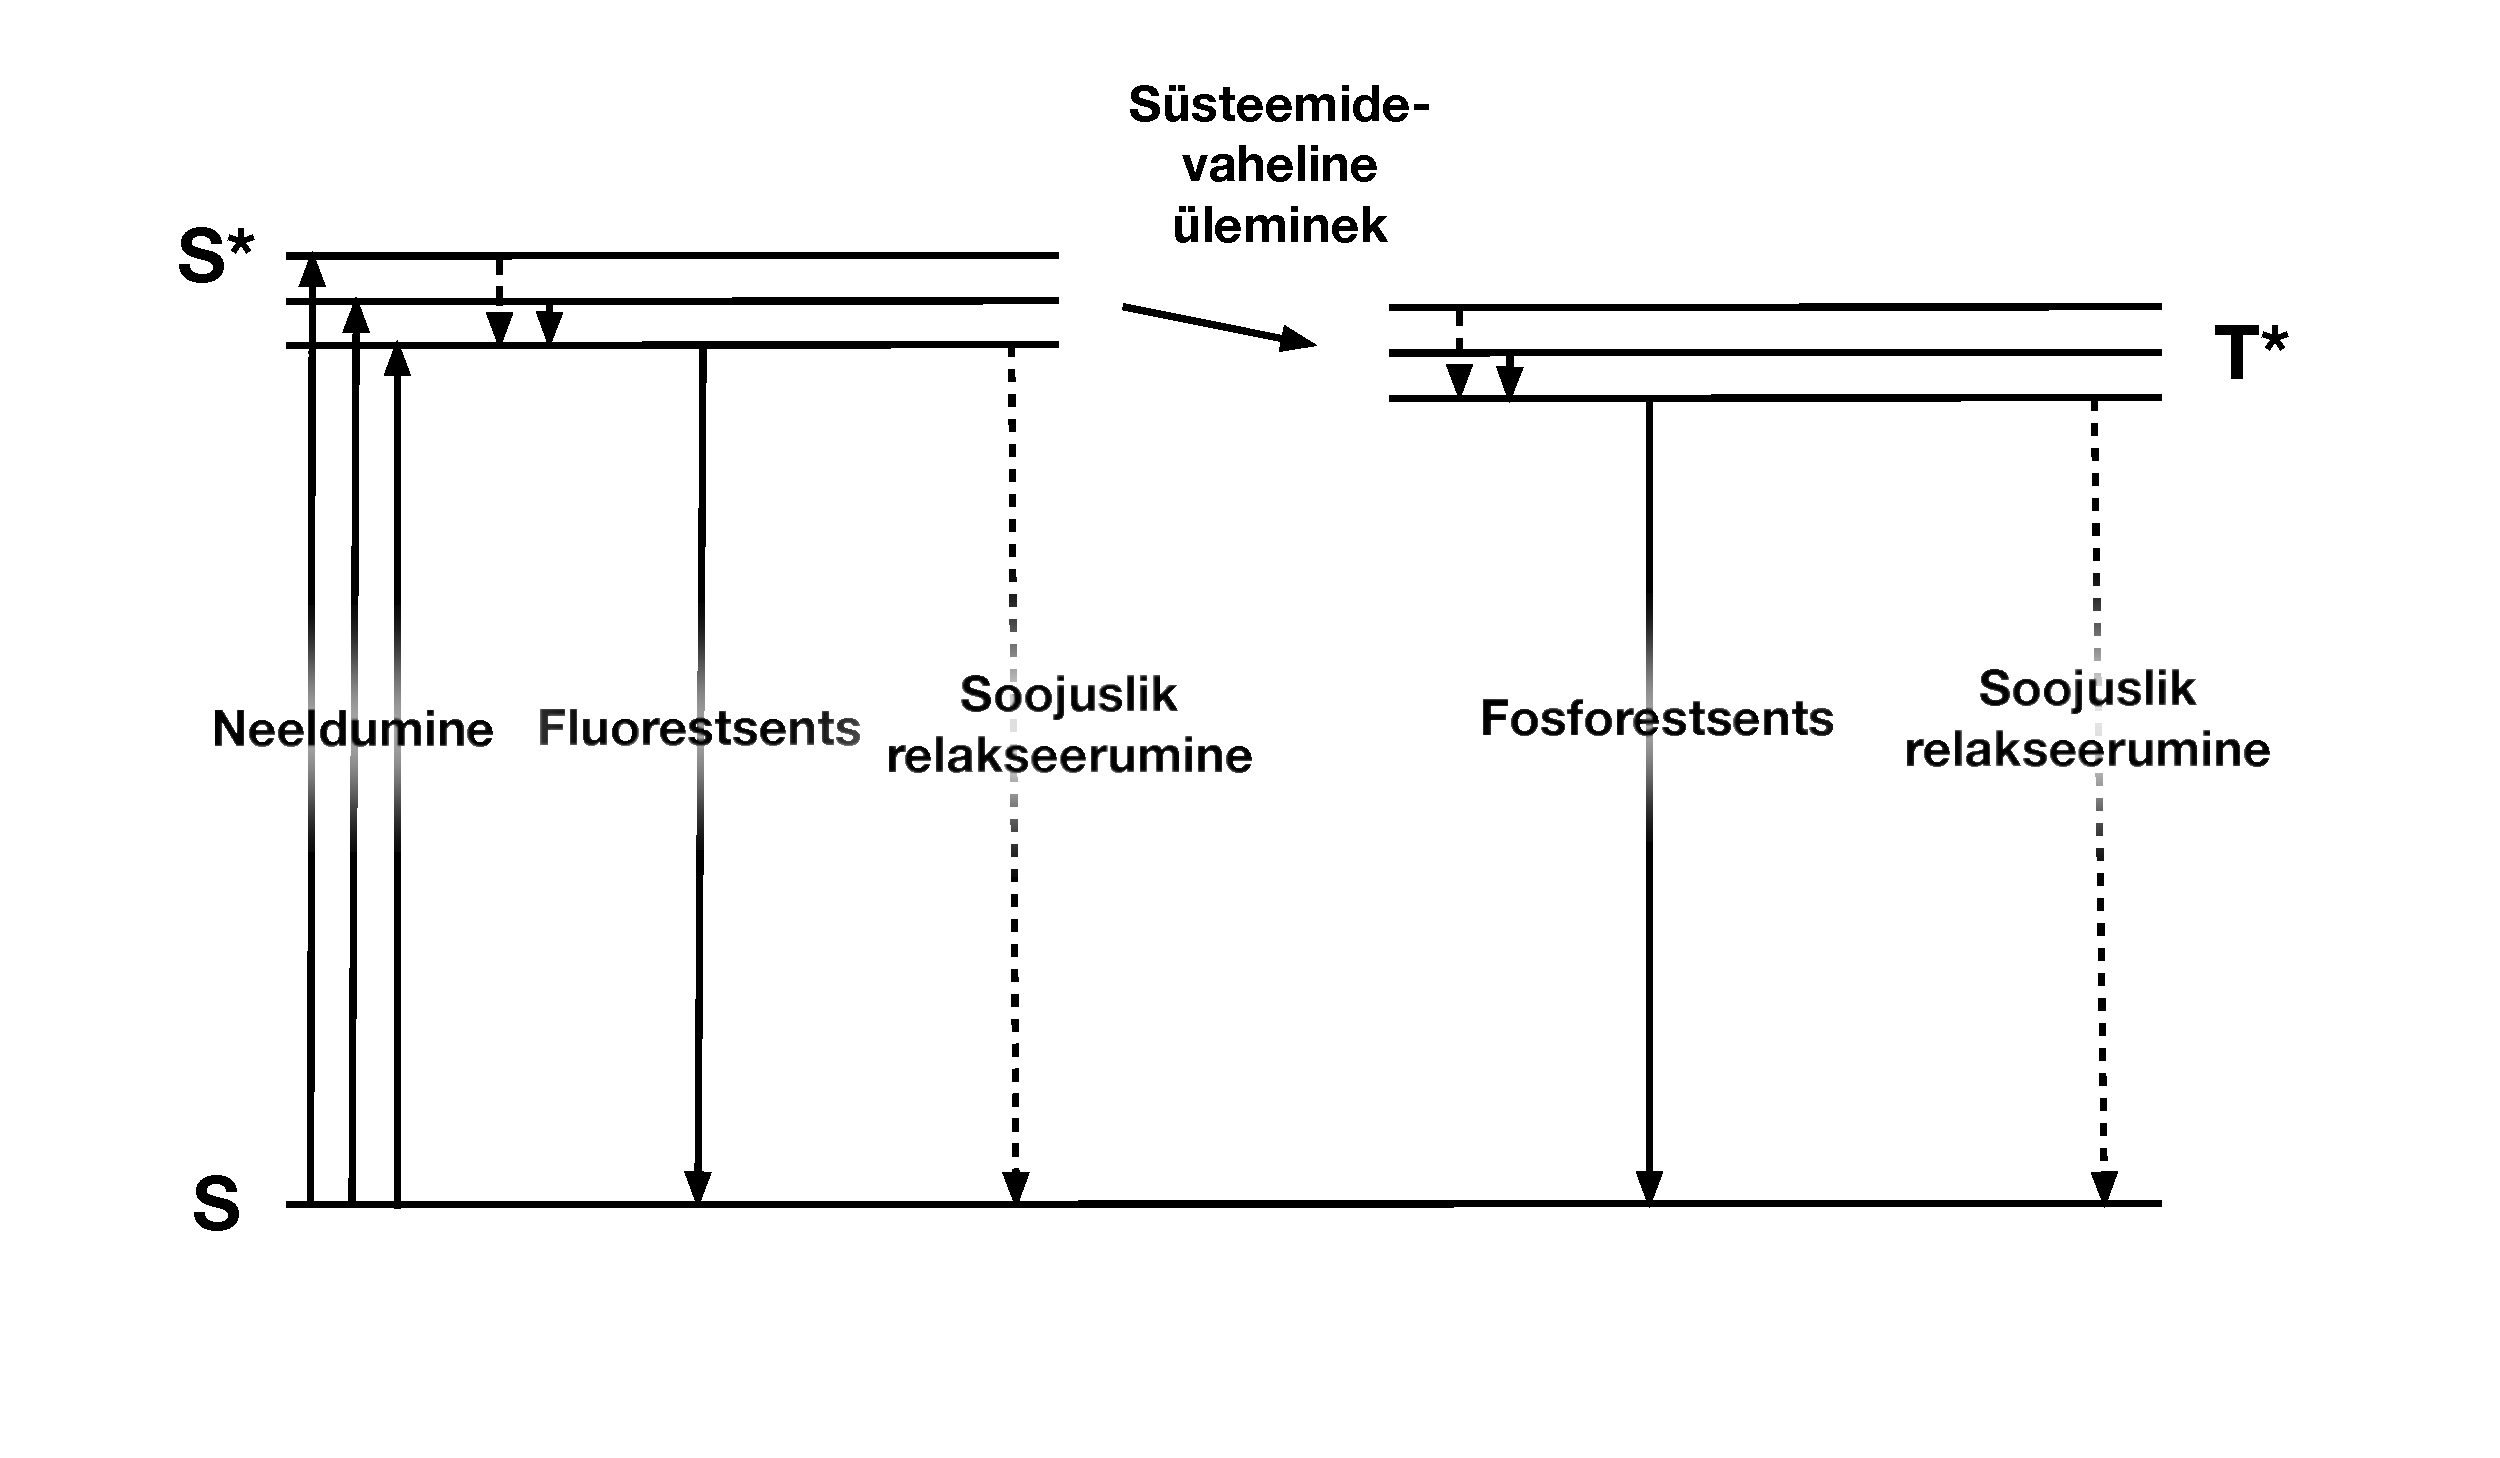
\includegraphics[width=\textwidth]{figures/jablonski.pdf}
    \caption{\label{jablonski}Lihtsustatud Jablonski diagramm. S vastab ühendi ergastamata põhiolekule, S$^*$ ja T$^*$ tähistavad vastavalt singletset ning tripletset ergastatud olekut. Punktiirjoonega on tähistatud mittekiirguslikud protsessid (nendega ei kaasne footoni neeldumist või eraldumist).}
\end{figure}

\subsection{Viitamine}

Viidata saab nii valemitele (vt valemeid \ref{gauss} ja \ref{gaussmagnet}), tabelitele (vaata tabel \ref{tabel}) kui ka joonistele (vt joonis \ref{jablonski}).

Viidata saab ka artiklitele \cite{iupac} ning raamatutele \cite{Atkins2005, Lakowicz2006}.